\chapter{Einleitung}
\paragraph{}
Die ckc group ist ein von Christian Krentel im Jahr 1989 gegründeter IT- und Business-Consulting-Anbieter in Braunschweig. Sie gehört in dem Bereich zu den führenden Unternehmen Deutschlands. In den Standorten Braunschweig, Berlin, Darmstadt, Hamburg, Dortmund und München beschäftigt sie rund 400 Mitarbeiter\fcitetitle{Mitarbeiterzahl}.
\paragraph{}
Hauptbranchen des Unternehmens sind die Automobilindustrie samt Zulieferer sowie Banken, Versicherungen, Luft- und Raumfahrt, Retail, Transport und Logistik. Die Kernkompetenz von ckc liegt im Bereich der IT nicht nur auf der 
Softwareentwicklung, sondern zu Teilen zusätzlich auf der Managementberatung.

\section{Projektbeschreibung}
\paragraph{}
Das ”Sisyfox” Projekt wird entworfen, um für firmeninterne Events (z.B. Seminare, Konferenzen, Sommerfeste, etc.) eine Attraktion zu bieten, die nicht nur mit Spaß verbunden wird, sondern aus der sich auch ein Lernwert ergibt. 
Das Spiel stellt in einer vereinfachten Form den Mythos des Sisyphos und sein immerwährendes Scheitern gamifiziert\fcitetitle{Gamifizierung} dar. Den Mitarbeitern soll dabei der Umgang mit dem Erlebnis des Scheiterns näher gebracht werden. Außerdem soll diese Gamifizierung zu einer Motivationssteigerung führen.
\paragraph{}
Der Charakter im Spiel wird mit einem Aufbau, auf dem ein 1.20m großer Ball als Steuerkugel\footnote{Wie in einem Kugellager.} befestigt ist, vom Spieler gelenkt. Dafür steht der Aufbau vor dem Spieler auf dem Boden. 
Die Kugel kann durch den Aufbau mit den Händen auf der Stelle bewegt werden. Die Sensordaten des Aufbaues werden direkt an den Computer übermittelt und müssen in der Steuerung umgesetzt werden. 
\paragraph{}
Die Aufgabe in dem Projekt besteht darin, die Steuerung für den Charakter im Spiel zu programmieren. Diese wird in der Programmiersprache C\# geschrieben, damit sie in der Spieleentwicklungsumgebung ”Unity” als Skript in das vorhandene Projekt eingebunden werden kann. Hierbei muss auf eine intuitive Steuerung geachtet werden, da die Attraktion einer großen Zielgruppe zur Verfügung gestellt werden soll. Die Intuitivität\footnote{Je leichter es ist sich die Bedienung der Steuerung anzueignen, desto höher ist die Intuitivität.} soll durch eine leicht erlernbare Steuerung sowie eine deutliches visuelles Feedback realisiert werden. Im Projekt vorhanden sind bereits sämtliche Modelle, Animationen sowie Sounds und Hintergrundmusik, aber auch schon einzelne, von mir früher programmierte Skripte, die sich z.B. um das Benutzerinterface kümmern. Die benötigten Daten für die Steuerung des Charakters werden von einer Trackballmaus zum Computer übertragen und müssen dort in die Bewegung umgesetzt werden. Außerdem muss im Rahmen der Projektarbeit bestimmt werden, wie sich der Charakter in der virtuellen Welt verhält, in welchen Situationen der Spieler das Spiel vorzeitig verlieren kann und ab welchem Zeitpunkt das Spiel gewonnen ist.

\section{Projektziel}
\paragraph{}
Mit dem Projekt soll eine gewisse Hartnäckigkeit, gefolgt von gesteigerter Motivation durch Erfolgserlebnisse bei den Mitarbeitern, sowie Besuchern von Firmenfesten und anderen Events erzielt werden. Der Benutzer wird mit jeder gespielten Runde vor die Aufgabe gestellt, eine scheinbar unerreichbare Hürde zu überwinden. Er wird viele Versuche brauchen, um den Gipfel zu erreichen. Der spielerische Aspekt sorgt unweigerlich dafür, dass der Benutzer leichter mit häufigen Niederlagen umgehen kann, um anschließend den anfangs weit entfernten Berg erneut herauszufordern. Sobald der Spieler am Gipfel angekommen ist, gibt es auditive und visuelle Erfolgsmeldungen. Dazu erscheint eine Anzeige, wie lange der Weg zur Bergspitze gedauert hat, damit der Spieler sich mit anderen messen kann und ein Wettkampfgefühl entsteht.

\section{Projektabgrenzung}
\label{Projektabgrenzung}
\paragraph{}
Im Projekt sind bereits ein Spielehauptcontroller sowie eine Animations- und Bewegungssteuerung vorhanden.
Der Hauptcontroller sorgt für die Verwaltung der Grundstatus\footnote{Die vier Status sind in aktiv, spielend, gewonnen und verloren eingeteilt.} im Spiel. Außerdem speichert er die wichtigsten Variablen, wie unter anderem Spieldauer oder die Höhe abweichend vom Fuß des Berges. Es wird lediglich ein Verweis via Assoziation in der Charaktersteuerung eingebunden, damit z.B. die Höhendaten kommuniziert werden können.

\chapter{Projektplanung}
\section{Projektphasen}
\paragraph{}
Für die Umsetzung des Teils des Projekts stehen insgesamt 70 Stunden zur Verfügung. Die Entwicklung wurde vor Beginn des Projekts auf die verschiedene Projektphasen aufgeteilt. In der folgenden Tabelle \tref{tab:Zeit} lässt sich die grobe Zeitplanung ablesen.\\
\begin{table}[h]
\centering
\begin{tabular}{lr}
\rowcolor{ckcGreen}\textbf{Projektphase} & \textbf{Geplante Zeit}\\
\hline
Ist-Analyse & 6 Std\\
\rowcolor{odd}Soll-Konzept & 11 Std\\
Implementierung & 24 Std\\
\rowcolor{odd}Integration in das Unityprojekt &  8 Std\\
Testen und Fehlerbehebung & 11 Std\\
\rowcolor{odd}Dokumentation & 10 Std\\
\hline
\hline
\rowcolor{ckcGreen}\textbf{Gesamt} & \textbf{70 Std}\\
\end{tabular}
\caption{Grobe Zeitplanung}
\label{tab:Zeit}
\end{table}

\section{Ressourcenplanung}
Es werden alle verwendeten Ressourcen wie Hard- und Software in einer Übersicht im Anhang in \fullref{Abb:Ressourcen} aufgeführt. Um möglichen Aufwand für Software so gering wie möglich zu halten, wurde darauf geachtet, kostenfreie sowie Open Source Software zu benutzen.

\chapter{Analysephase}
\section{Ist-Analyse}
\paragraph{}
In dem Spiel gibt es viele kleine Details, welche über das Einbinden von Scripten und das Platzieren von 3D-Modellen realisiert werden. Dazu gehört zunächst die Spielkarte, auf der sich der Charakter bewegt. Diese wurde von anderen Teammitgliedern erstellt, mit 3D-Modellen wie z.B. Bäumen, Sträuchern oder Gesteinsbrocken bestückt und in das Projekt implementiert. Zusätzlich wurden 3D-Modelle von Wolken und Vögeln erstellt, die sich im Kreis um den Hauptberg bewegen\footnote{Die Bewegung wird von einem Script gesteuert.}.
Die Spielfigur namens \q{Sisyfox} gehört zu den schon erstellten 3D-Modellen und wurde ebenfalls schon mit einer vollständigen Animation versehen. Diese Animation hat jedoch nichts mit der eigentlichen Bewegung des Charakters zu tun. Sie zeigt lediglich visuell eine Laufbewegung an, die aber nicht für eine Positionsverschiebung sorgt. 
Wie in \autoref{Projektabgrenzung} \nameref{Projektabgrenzung} bereits erwähnt, ist der Hauptcontroller, als eines von vielen Scripten, schon vorhanden. Weitere wichtige Scripte sind die Kamerasteuerung, sämtliche Animationsscripte, eine Höhenmeteranzeige und ein Arduinokommunikationsscript, welches eine Verbindung zu einer Hardwarekonstruktion namens \q{Arduino\fcitetitle{Arduino}} aufbaut. Letztes sorgt dafür, dass sich relativ zur Höhe auf der sich der Charakter befindet, ein angeschlossener Ventilator stärker dreht und eine Nebelmaschine kurz vor Erreichen des Gipfels anspringt.

\section{Anforderungsanalyse}
\paragraph{}
Um die Positionsverschiebung des Spielecharakters zu implementieren, muss eine Steuerung geschrieben werden. Diese soll von dem Nutzer kontrolliert werden. Das bedeutet, dass der Nutzer Eingaben tätigt und die Steuerung dafür sorgt, dass es ein visuelles Feedback gibt. Hierbei muss innerhalb der Steuerung auf vorher festgelegte Niederlage- und Gewinnbedingungen reagiert und zusätzlich eine möglichst realistische und damit intuitive Bewegung ermöglicht werden. In der Entwurfsphase wird das genauere Vorgehen einschließlich einer Programmarchitekturauswahl hinsichtlich der gestellten Anforderungen erläutert.

\section{Qualitätsanforderungen}
\paragraph{}
Das Spiel und der dazu geschriebene Code muss folgenden Qualitätsanforderungen entsprechen. \\
Im Code muss ein sauberer Schreibstil gepflegt werden, um bei Wartungen oder Veränderungen den Aufwand gering zu halten. Dafür werden für jede Methode Kommentare verfasst, die die grundlegende Funktion beschreiben. Des Weiteren werden die einzelnen Funktionsweisen in Methoden von einander getrennt. Variablenamen müssen selbstsprechend benannt werden und bei Abweichung für Hilfsvariablen, darüber ein Kommentar mit einer kurzen Beschreibung geschrieben werden.
Nach dem Fertigstellen einzelner Methoden wird ein manueller Test der implementierten Funktion durchgeführt. Das Spiel wird gestartet und die Funktion ausprobiert.

\chapter{Entwurfsphase}
\section{Zielplattform}
\paragraph{}
Zur Auswahl standen die IDEs\footnote{eng: integrated development environment, de: Integrierte Entwicklungsumgebung} \q{Unity 3D Engine} und \q{Unreal Engine 4}. Gewählt wurde die Unity Engine, da in dieser gegenüber der Unreal Engine deutliche Vorkenntnisse vorhanden sind, die dann im Projekt für einen flüssigen Workflow sorgen. Ein weiterer Grund ist das sehr einfache und intuitive Einbinden von Gameobjekten\footnote{\q{Gameobjekte} sind die Grundbausteine von jedem Unity Spiel und können verschiedene Komponenten aufnehmen, um damit den unterschiedlichen Aufgaben eines Spiels gerecht zu werden.} und deren angebundenen Scripten.

\section{Architekturdesign}
\paragraph{}
Für den Architekturaufbau standen das \q{Model-View-Controller-} (MVC) und das \q{Presentation-Abstraction-Control-Muster} (PAC) zur Auswahl.
\paragraph{}
Das MVC Muster (Siehe Schema \fullref{Abb:MVC}) besteht grundsätzlich aus drei Strukturen, die unterschiedliche Ebenen im Programmaufbau darstellen.
Diese unterteilen sich in \q{Modell-}, \q{View-} und \q{Controller-Ebene}. Die Unterteilung dient hierbei dem Zweck, dass jede Ebene flexibel und unabhängig von den Anderen verändert, ersetzt oder erweitert werden kann. 
Das Modell beinhaltet die Daten, die für die Anzeige nötig sind. Über die View-Ebene werden die Daten aus dem Modell dem Benutzer angezeigt und des Weiteren mögliche Benutzereingaben entgegengenommen. Wenn sich Daten im Modell ändern wird im Regelfall die View-Ebene mithilfe eines Beobachters\footnote{Der Beobachter meldet sich bei der View-Ebene, sobald sich Daten im Modell ändern.} benachrichtigt, sodass sich die View aktualisieren kann. Die entgegengenommen Benutzereingaben werden von dem Controller übernommen und verarbeitet. In dem objektorientierten Ansatz führt der Controller Methoden im Modell aus, damit die Aktionen des Benutzers wirksam werden. Außerdem kann der Controller die View direkt manipulieren, um z.B. die angezeigten Eingabemöglichkeiten zu verändern. 
\paragraph{}
Für den alternativen Ansatz, in dem man ein System in verschiedenen Einzelteilen erstellt, benötigt man ein Muster, das jede Aufgabe in einem anderen Teil des System, abbildet. Dadurch wird hohe Flexibilität ermöglicht, die sich auch im Wartungsaufwand widerspiegelt.
Im PAC Muster (Siehe Schema \fullref{Abb:PAC}) teilt man das System in zwei Richtungen auf, zunächst in drei Einheiten, die grafische Oberfläche, eine Kommunikationsschnittstelle und ein Datenmodell. Diese Einheiten ähneln dem MVC-Muster.
\paragraph{}
Darüber hinaus teilt sich das Architekturmuster hierarchisch auf sogenannte \q{Agenten} auf.
Diese Agenten werden auf drei Schichten verteilt, auf \textit{Top-Level-}, \textit{Intermediate-Level-} und \textit{Bottom-Level}-Agenten. Den \textit{Top-Level}-Agenten gibt es nur einmal im System, er übernimmt die globalen Aufgaben. Für die \textit{Bottom-Level}-Agenten ist eine möglichst in sich abgeschlossene Aufgabe vorgesehen. Die \textit{Bottom-Level}-Agenten können über implementierte Methoden in den \textit{Intermediate-Level}-Agenten mit dem \textit{Top-Level} kommuniziert.
\paragraph{}
In dem Projekt wird sich für eine einfache Variante des PAC-Musters entschieden. Der schon vorhandenen Hauptcontroller wird als Top-Level-Agent eingestuft und die Charaktersteuerung als eine Mischung aus Intermediate- und Bottom-Level-Agent. Die Steuerung wird über eine einfache Assoziation direkt mit dem Hauptcontroller kommunizieren können. Im nächsten Abschnitt wird der Entwurf eines Klassendiagrammes erläutert, in dem diese Herangehensweise umgesetzt wird.

\section{Entwurf der Benutzeroberfläche}
\paragraph{}
An der Benutzeroberfläche wird in dem Projekt nichts verändert. Es werden jedoch einige Daten von der Charakter Steuerung an den Hauptcontroller übermittelt, welche auf dem Bildschirm angezeigt werden. Im Anhang befindet sich eine Skizze (Siehe Anhang \fullref{Abb:UISkizze}) sowie ein Anzeigebild aus dem laufendem Spiel (Siehe Anhang \fullref{Abb:UIIngame}), in dem die wichtigsten Anzeigen eingetragen sind. Auf der Skizze befindet sich Punkt \q{A} oben links auf dem Bildschirm lokalisiert. An der Position wird eine weiße Bergsilhouette gezeigt, die sich relativ zur Charakterhöhe am Berg füllt. Die Charakterhöhe wird von der Charaktersteuerung ermittelt und an den Hauptcontroller für die Anzeige der Höhe und der Bergfüllanzeige übergeben. Gleich rechts daneben - Punkt \q{B} - zeigt die vergangene Zeit für den bisherigen Versuch an. In der Mitte des Bildschirms ist eine Höhenanzeige in Metern eingebaut (siehe Punkt \q{C}). Diese erscheint alle 150 Höhenmeter und gibt den derzeitigen Zwischenstand an. Anschließend verschwindet sie wieder. Als letzten Punkt auf der Skizze ist die Charakterposition eingezeichnet.
\paragraph{}
In der \fullref{Abb:UIIngame} sind alle auftretenden Benutzerinterface Anzeigen im Spiel dargestellt.

\section{Geschäftslogik}
\label{Geschaeftslogik}
\paragraph{}
Zunächst werden die Anforderungen an die Charaktersteuerung festgelegt, damit daraus ein Klassendiagramm entstehen kann. Das Klassendiagramm kann im Anhang in \fullref{Abb:KlassendiaMain} eingesehen werden. Die Steuerung muss als Hauptaufgabe die Mausinformationen sowie deren Bewegungsrichtung ermitteln und in eine Bewegung der virtuellen Kugel übersetzen. Um das zu realisieren, muss die aktuelle Mausbewegungsrichtung gespeichert werden. Daraus wird ein Richtungsvektor ermittelt. Der Vektor muss anschließend mit der einer spezifischen Geschwindigkeit multipliziert werden, damit die Beschleunigung entsteht. Nun ist ein Problem entstanden. Die Richtung, in die die Maus bewegt wurde, kann nicht direkt auf die Bewegungsrichtung der Kugel addiert werden, da die Kugelbewegung auf dem 3D Weltkoordinatensystem\footnote{Das Koordinatensystem ist statisch. Die Kugelbewegung ist, obwohl sie visuell nach vorne rollt, möglicherweise abweichend davon.} liegt und die Mausbewegung auf dem Bildschirmkoordinatensystem.

\begin{wrapfigure}{r}{0.5\textwidth}
\begin{center}
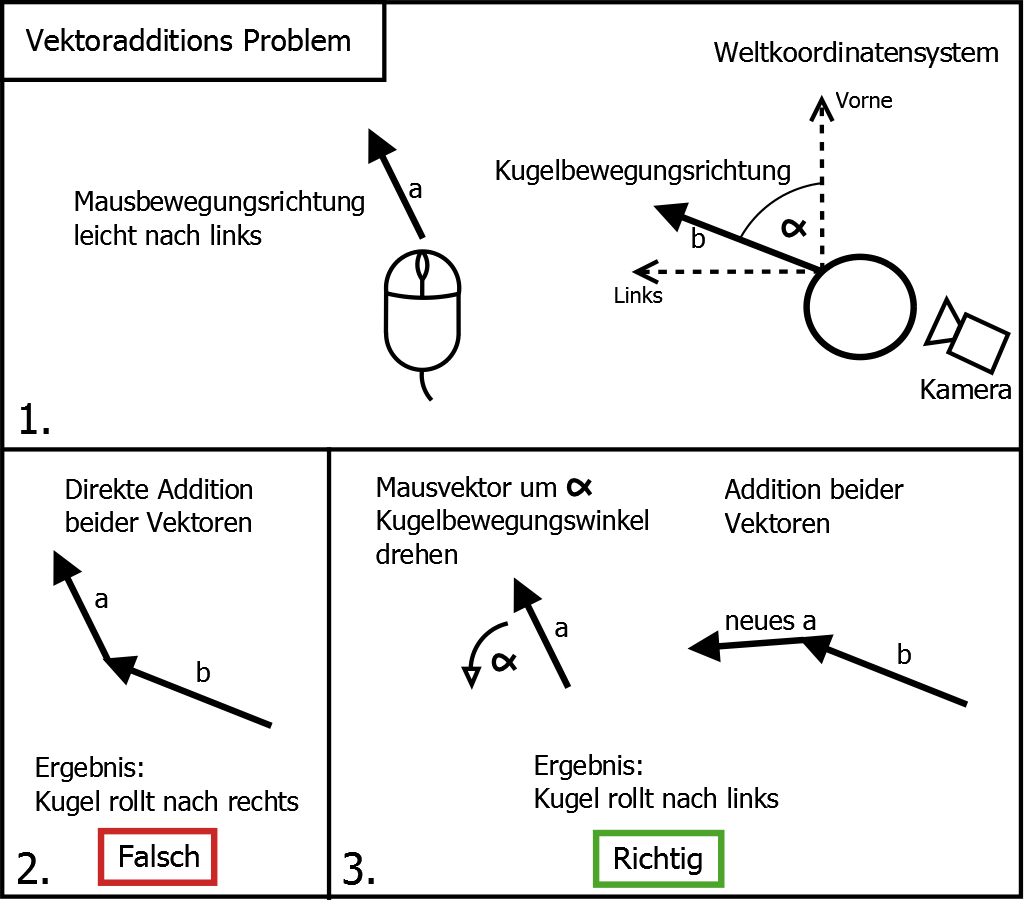
\includegraphics[scale=0.28]{Bilder/Diagramme/KoordinatensystemProblem.png}
\end{center}
\begin{footnotesize}
\caption{Koordinatensystem Problem}
\label{Abb:KoordinatensystemProblem}
\end{footnotesize}
\end{wrapfigure}

Ein Beispiel (Siehe auch \autoref{Abb:KoordinatensystemProblem}: Das Eingabemedium wird vom Benutzer nach links vorne geschoben, daraus entsteht ebenfalls eine Mausbewegung nach links vorne. Das ist der Vektor \q{a} in \autoref{Abb:KoordinatensystemProblem} bei Punkt [1]. Vektor \q{b} bezeichnet die aktuelle Kugelbewegung innerhalb des Weltkoordinatensystems. Für den Benutzer rollt die Kugel nach vorne, da die Kamera immer hinter dem Betrachter in Bewegungsrichtung schauend steht. Im Weltsystem ist die Rollrichtung jedoch ein Vektor, der von der Weltrichtung \q{vorne} abweicht. Das heißt, wenn jetzt wie in Punkt [2] die beiden Vektoren ohne Vorbehandlung addiert werden, die Kugel nicht wie gewünscht nach links, sondern nach rechts rollt. Um die unbeabsichtigte Richtung zu korrigieren, muss der Mausbewegungsvektor \q{a} um den Winkel \alp{} aus Punkt [1], der die Abweichung des Welt \q{vorne} Vektors von der Kugelbewegungsrichtung darstellt, gedreht werden. Anschließend kann der \q{neue a} Vektor wie in Punkt [3] auf den Kugelvektor \q{b} addiert werden. Daraus resultiert jetzt die erwartete Bewegungsrichtung.
\paragraph{}
Ergänzend sollen vorher festgelegte Mechanismen überprüfen, in welchen Situationen der Spieler das Spiel gewinnt oder verliert. Dieser Zustand oder auch Status des Spiels wird vom Hauptcontroller verwaltet (Siehe Statemachine Anhang \fullref{Abb:SMStatus}). Der Status geht vom \textit{inaktiv}\footnote{Im inaktiv Status verweilt das Spiel solange, wie es keine Benutzerinteraktion gibt.} Status über in den \textit{laufend} Status, welcher je nach Spielweise in \textit{gewinnen} oder \textit{verlieren} endet. Gewinnen wird der Spieler, wenn er am Gipfel des Berges angelangt ist und dort in eine Triggerbox\footnote{Ein Trigger ist in dem Fall eine unsichtbare Box mit Kollisionserkennung an den Außenseiten, die ein Kollisionsevent erzeugt. Das Event löst eine Funktion beim kollidierenden Objekt aus.} (Siehe auch \fullref{Abb:GewinnTrigger}) hineinläuft und somit den \textit{gewonnen} Status erreicht. Der Niederlage-Mechanismus funktioniert ähnlich. Hierfür wurde festgelegt, dass bei Berührung eines Baumes (Siehe auch \fullref{Abb:BaumTrigger}) oder Felsbrockens das Spiel verloren sein soll. Dafür werden diese ebenfalls mit einem Trigger versehen, der den \textit{verloren} Status auslöst.
\paragraph{}
Zusätzlich soll der Kugel eine möglichst realistische Physik gegeben werden. Das heißt, dass der Charakter nicht in der Lage sein soll, die Kugel seitlich an einem Abhang entlang zu rollen, ohne dass sie ihm zur Seite weg rollt und er die Runde verliert. Diese Mechanik ist in \autoref{Abb:VerlierWinkelSeitlich} visualisert. Der Benutzer kann als Reaktion versuchen den Charakter unter die Kugel zu manövrieren, sodass die Steigung vor ihm liegt und nicht seitlich.

\begin{wrapfigure}{l}{0.525\textwidth}
\begin{center}
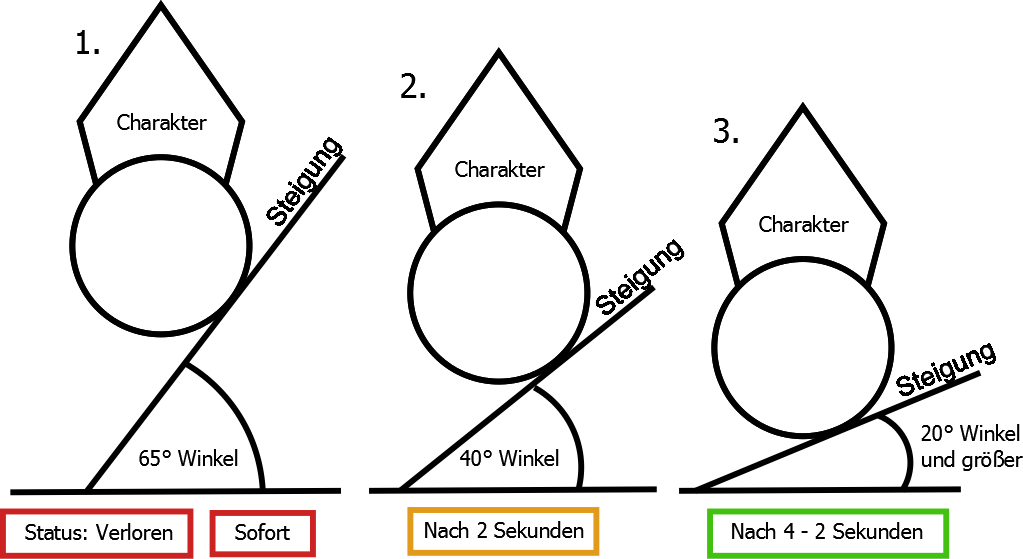
\includegraphics[scale=0.17]{Bilder/Diagramme/VerlierWinkelSeitlich.png}
\end{center}
\begin{footnotesize}
\caption{Bedingungen bei seitlichem Neigungswinkel}
\label{Abb:VerlierWinkelSeitlich}
\end{footnotesize}
\end{wrapfigure}

Dann kann der Charakter die Kugel festhalten. Bei einem seitlichen Neigungswinkel von über 65\cc, wie bei Punkt [1], verliert der Spieler sofort das Spiel. Liegt der Winkel, wie in Punkt [2], zwischen 40\cc und 65\cc, dann hat der Spieler 2 Sekunden, um seine Spielfigur zu richten. Auf einem Hang, wie in Punkt [3], mit einem Neigungswinkel zwischen 20\cc und 40\cc hat der Spieler abhängig vom Winkel vier bis zwei Sekunden Zeit die Spielfigur zu richten. Wie angesprochen kann die Spielfigur die Kugel an beliebig steilen Steigungen festhalten, solange sie sich unter\footnote{\q{Unter} bedeutet, dass der Spieler gerade auf die Steigung zuläuft.} der Kugel befindet. Befindet sich der Charakter auf der anderen Seite (\q{über} der Kugel), dann ist die Kugel ebenfalls bei einem Winkel von 65\cc verloren.
\paragraph{}
Als weitere Funktion der Steuerung soll der Charakter, wenn er durch einen Busch läuft, verlangsamt werden. Hierzu muss für jeden Busch ein weiterer Trigger (Siehe auch \fullref{Abb:BuschTrigger}) hinzugefügt werden.

\section{Maßnahmen zu Qualitätssicherung}
\paragraph{}
Um die Qualität der umzusetzenden Steuerung zu gewährleisten, wird während der Implementierung nach jeder Einbindung einer neuen Funktion, ein manueller Test durchgeführt. Die neue spezifische Funktion wird anhand einer augenscheinlichen Ausführung und Debug-Informationen\footnote{Die Debug-Informationen werden \q{hard-coded}. Das bedeutet, dass die Informationen zum erfolgreichen Erreichen des Codeabschnittes direkt in den Code geschrieben werden und dort nach erfolgreichem Test gelöscht werden.} begutachtet. Daraus wird geschlussfolgert, ob die Implementierung erfolgreich eingesetzt wurde.

\chapter{Implementierungsphase}
\section{Implementierung der Klassenstruktur}
\paragraph{}
Am Anfang werden die beiden Klassen \q{SphereController} und \q{stSphere} erstellt. Die Steuerung des Kugel wird hier \q{SphereController} genannt, da es bereits einen \q{CharacterController} gibt. Dieser ermittelt den aktuellen Stand der Animation der Spielfigur und deren Position hinter der Kugel. Die Bezeichnung ist daher passend, weil sich die Steuerung im Endeffekt um die Bewegung der Kugel oder auch \q{Sphere} kümmert. 
\paragraph{}
In die Klasse \q{stSphere} werden alle spezifischen Daten der Sphere abgelegt. Im Anhang ist die vollständige Klasse in \fullref{Abb:stSphere} abgebildet. Für sie wurde die statische Variante gewählt, da es im Spiel nur eine einzige Kugel gibt und sich deren Eigenschaften nicht verändern. So muss im \q{SphereController} kein Objekt der Kugel erstellt werden. In der Steuerung kann einfach via \q{stSphere.Variablename} auf die Attribute der Kugel zugegriffen werden. Alle Variablen der \q{stSphere} Klasse sind nur mit \textit{gettern}\footnote{Ein \textit{getter} ermöglicht eine Anpassung der Rückgabefunktion der zugehörigen Variable.} versehen, damit es nicht die Möglichkeit gibt durch einen anderen Script die Werte zu verändern\footnote{Der Wert könnte mithilfe eines \textit{setters} von außerhalb verändert werden. Der wurde hier weggelassen.}. Die eingesetzten Variablen sind direkt initialisiert. Die Werte ergeben sich aus mehreren manuellen Tests und anschließender Optimierung an die subjektiv beste Spielerfahrung. In der Klasse finden sich, die in \autoref{Geschaeftslogik} \nameref{Geschaeftslogik} festgelegten Winkelbedingungen unter \q{InstantLossAngle}, \q{MiddleLossAngle} und \q{LowLossAngle} wieder. 
\paragraph{}
Für die \q{SphereController} Klasse werden zunächst die Verweise und Abhängigkeiten zu den anderen Scripten geschaffen. Der \q{GameController} Script übergibt sich selbst bei der Instanzierung\footnote{Instanzierung heißt bei Unity, dass ein Objekt als Kopie eines \textit{Prefabs} in der 3D-Welt erstellt wird. Ein \textit{Prefab} ist ein zuvor erstelltem Spielobjekt mit angebundenen Komponenten, in dem Fall die Spielefigur mit Kameraobjekt und Kugelobjekt. An das Kugelobjekt ist der \q{SphereController} angebunden. Die Unity Ansicht kann in \fullref{Abb:SphereInspector} gesehen werden.} des Spielerobjektes an den Sphere Script. In  der Start Methode des \q{SphereController} wird der Verweis zu dem \textit{Transform}\footnote{Das Transform ist eine Komponente eines Gameobjektes und enthält dazu die Positions-, Rotations- und Skalierungsdaten. } sowie zu dem \textit{Rigidbody}\footnote{Das Rigidbody ist eine Komponente eines Gameobjektes und sorgt für Physikbeachtung des Objektes. Dazu gehört z.B. das Reagieren auf die Schwerkraft oder Kollidieren mit anderen Gameobjekten. Zum Kollidieren wird zusätzlich eine \q{Collider}-Komponente benötigt.} der Kugel erstellt. Im folgenden ist ein Ausschnitt der Startfunktion zu sehen.

\lstinputlisting[caption={Startfunktion}]{Code/startVerweise.txt}

\section{Implementierung der Geschäftslogik}
\paragraph{}
Im Anschluss an die Implementierung der Klassenlogik wird sich der Geschäftslogik gewidmet. Der \q{SphereController} Script hat eine Update Funktion, die von der Engine\footnote{Die Engine arbeitet im Hintergrund des Spiels und ruft unter anderem die Start und Update Funktionen in Scripten auf. Außerdem kümmert sie sich auch um die grafische Darstellung vom} vor jedem Frame\footnote{Ein Frame ist ein angezeigtes Bild während das Spiel läuft. Das Spiel läuft mit ca. 60 Frames pro Sekunde.} aufgerufen wird. Dort wird sich je nach Hauptsteuerungsstatus entschieden, welche Funktionen ausgeführt werden. Außerdem wird in jedem Update Aufruf die Mausbewegungsrichtung\footnote{Die Mausbewegung wird durch das physische Eingabemedium erzeugt.} zwischengespeichert. Die Methode \q{GetAxis} gibt einen Wert zwischen -1 und 1 für die angegebene Achse zurück, der, wenn \textit{mouseX} und \textit{mouseY} zu einem Vektor zusammengefasst werden, den Richtungsvektor symbolisiert.

\lstinputlisting[caption={Updatefunktion}]{Code/updateFunc.txt}

\paragraph{}
Die in der Updatefunktion aufgerufene \textit{State0{\_}Idle} Methode beinhaltet das Verhalten der Kugel im inaktiven Zustand. Dort wird abgefragt, ob die \textit{mouseX} oder \textit{mouseY} Variablen einen Wert anders als 0 hat, um eine Bewegung des Eingabemediums festzustellen. Sobald die Kugel vom Benutzer bewegt wird, gibt der \q{SphereController} dem \q{GameController} Bescheid, dass das Spiel nun in den nächsten Zustand (Siehe auch \fullref{Abb:SMStatus}) übergehen kann.

\lstinputlisting[caption={\q{Idle} Funktion}]{Code/State0Idle.txt}

\paragraph{}
Im Anschluss geht es an die Umsetzung der in \autoref{Geschaeftslogik} \nameref{Geschaeftslogik} genannten Problemlösung der Vektorberechnung. Es wird die \textit{State1{\_}Running} Funktion erstellt. Am Anfang steht die Berechnung des Winkels für die Drehung des Mausvektors. Dieser ist in der Variable \textit{angle} abgelegt. \textit{Vector.Angle} ermittelt den Winkel zwischen \textit{Vector.forward} und der aktuellen Bewegungsrichtung \textit{new Vector( velocity.x, 0, velocity.z )}.

\lstinputlisting[caption={\q{Running} Funktion Teil 1}]{Code/State1RunningTeil1.txt}

\paragraph{}
Danach kann aus \textit{mouseX} und \textit{mouseY} der Mausvektor bestimmt werden. Solange die Geschwindigkeit der Kugel kleiner dem, in der Klasse \q{stSphere} festgelegten Wert ist, wird dem Vektor die \textit{mouseY} oder auch Schubkraftvariable hinzugefügt. Ansonsten kann im Endeffekt nur gelenkt und nicht geschoben werden, da die \textit{mouseX} nur für die Richtungsänderung zuständig ist. Die Variable \textit{angle} wird mit Hilfe der vorgegebenen \textit{Quaternion.AngleAxis} Methode auf die Mausbewegung multipliziert damit diese korrekt gedreht ist.

\lstinputlisting[caption={\q{Running} Funktion Teil 2}]{Code/State1RunningTeil2.txt}

\paragraph{}
Im nächsten Abschnitt wird die Neigungswinkel-Überprüfung betrachtet und umgesetzt. Anfangs werden die Winkel die sich im Moment unterhalb der Kugel befinden bestimmt. Dafür werden Raycasts\footnote{\q{Rays} sind Strahlen, die von der Engine in bestimmte Richtungen ausgesandt werden können und das Objekt, auf das sie treffen, zurückgeben.} benutzt, die ein Gameobjekt zurückgeben. Das Objekt beinhaltet eine Transformkomponente, die ihre genaue Position kennt. Und anschließend kann man mit jeweils zwei Raycasts, einerseits vor und hinter und andererseits rechts und links der Kugel, die Winkel zwischen den Treffern bestimmen. Im folgenden Codeausschnitt ist beispielhaft die Ermittlung des Winkels zwischen dem vorderen und hinterem Raycasttreffer dargestellt.

\lstinputlisting[caption={Neigungswinkel Überprüfung Teil 1}]{Code/SphereGradientCheckTeil1.txt}

\chapter{Abnahme- und Einführungsphase}
\section{Abnahme}
\section{Einführung}
\section{Dokumentation}

\chapter{Fazit}
\section{Soll-/Ist-Vergleich}
\section{Lessons Learned}
\section{Ausblick}
